\section{Altri Risultati}\label{sec:altri-risultati}
\subsection{Mean-field approximation}\label{subsec:app-mean-field-approximation}
    Qui vengono mostrate tutte le valutazione effettuate con il metodo di approssimazione del campo medio al variare di $k$.

    \begin{minipage}{\linewidth}
        \centering
        \begin{minipage}{0.45\linewidth}
            \begin{figure}[H]
            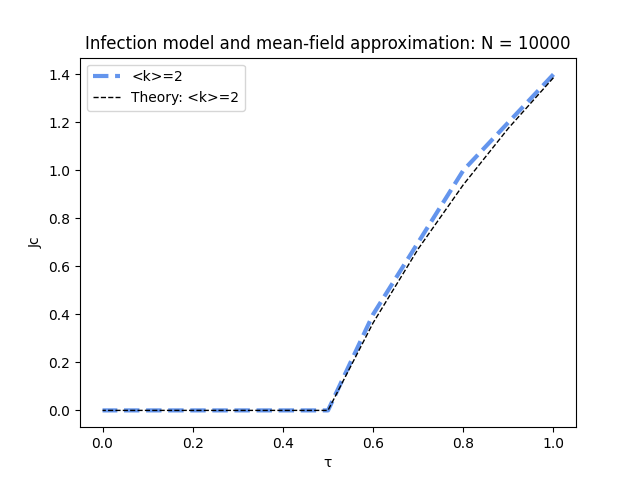
\includegraphics[width=\linewidth]{MF/k2-it10000}\caption{$k=2$: 10000 iterazioni}
            \label{fig:mf_k2}
            \end{figure}
        \end{minipage}
        \hspace{0.05\linewidth}
        \begin{minipage}{0.45\linewidth}
            \begin{figure}[H]
            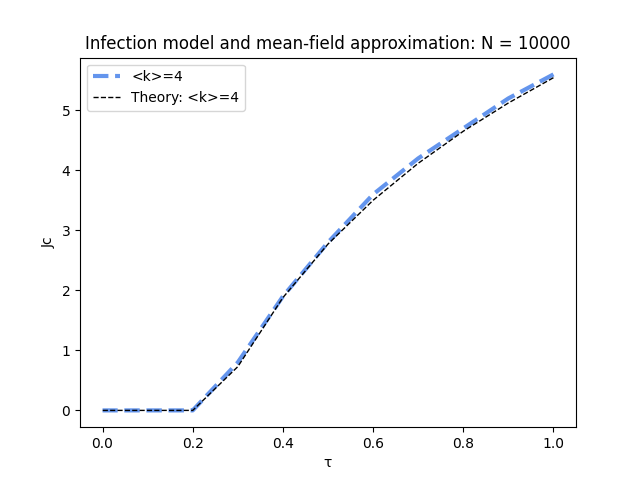
\includegraphics[width=\linewidth]{MF/k4-it10000}\caption{$k=4$: 10000 iterazioni}
            \label{fig:mf_k4}
            \end{figure}
        \end{minipage}
        \begin{minipage}{0.45\linewidth}
            \begin{figure}[H]
            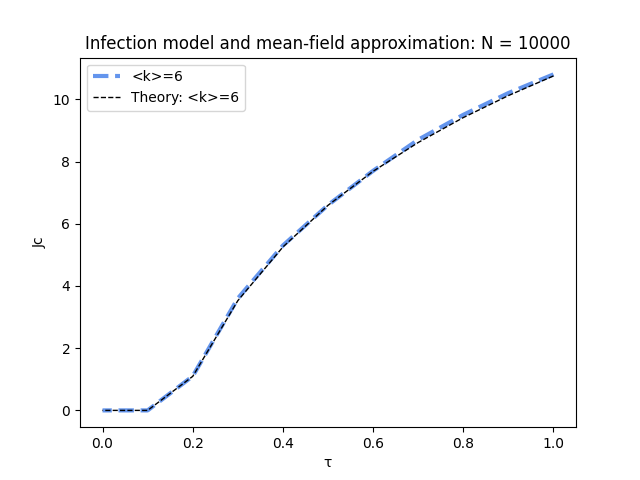
\includegraphics[width=\linewidth]{MF/k6-it10000}\caption{$k=6$: 10000 iterazioni}
            \label{fig:mf_k6}
            \end{figure}
        \end{minipage}
    \end{minipage}

\subsection{Simple percolation}\label{subsec:app-simple-percolation}
    \begin{figure}[H]
        \begin{minipage}{\linewidth}
            \centering
            \begin{minipage}{0.45\linewidth}
                \begin{figure}[H]
                \includegraphics[width=\linewidth]{SIM/Cycle-nodes50_it10000}\caption{Cycle}
                \label{fig:sim_cycle_nodes_50}
                \end{figure}
            \end{minipage}
            \hspace{0.05\linewidth}
            \begin{minipage}{0.45\linewidth}
                \begin{figure}[H]
                \includegraphics[width=\linewidth]{SIM/Poisson-k3_nodes50_it10000}\caption{Poisson: $k=3$}
                \label{fig:sim_poisson_k_3_nodes_50}
                \end{figure}
            \end{minipage}
            \begin{minipage}{0.45\linewidth}
                \begin{figure}[H]
                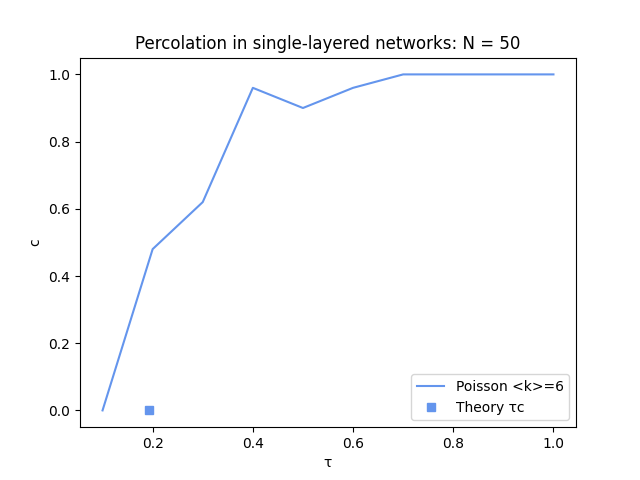
\includegraphics[width=\linewidth]{SIM/Poisson-k6_nodes50_it10000}\caption{Poisson: $k=6$}
                \label{fig:sim_poisson_k_6_nodes_50}
                \end{figure}
            \end{minipage}
            \begin{minipage}{0.45\linewidth}
                \begin{figure}[H]
                \includegraphics[width=\linewidth]{SIM/ScaleFree-k3_nodes50_it10000}\caption{Scale-Free: $k=6$}
                \label{fig:sim_scale_free_k_3_nodes_50}
                \end{figure}
            \end{minipage}
            \caption{Valutazione della probabilità di percolazione al variare della tipologia di grafo e del numero di nodi,
            con $n=50$ e 10000 iterazioni}
        \end{minipage}
    \end{figure}

    \begin{figure}[H]
        \begin{minipage}{\linewidth}
            \centering
            \begin{minipage}{0.45\linewidth}
                \begin{figure}[H]
                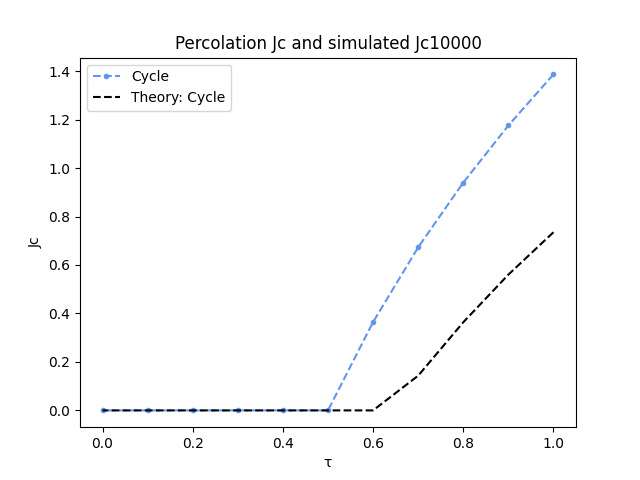
\includegraphics[width=\linewidth]{SIM/Cycle-nodes10000_it10000}\caption{Cycle}
                \label{fig:sim_cycle}
                \end{figure}
            \end{minipage}
            \hspace{0.05\linewidth}
            \begin{minipage}{0.45\linewidth}
                \begin{figure}[H]
                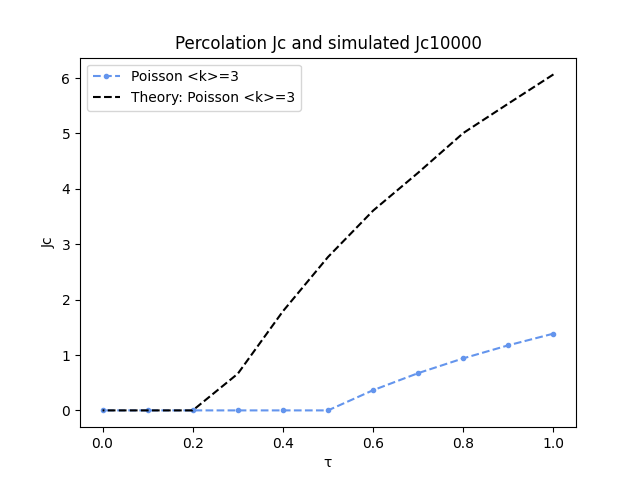
\includegraphics[width=\linewidth]{SIM/Poisson-k3_nodes10000_it10000}\caption{Poisson: $k=3$}
                \label{fig:sim_poisson_k_3}
                \end{figure}
            \end{minipage}
            \begin{minipage}{0.45\linewidth}
                \begin{figure}[H]
                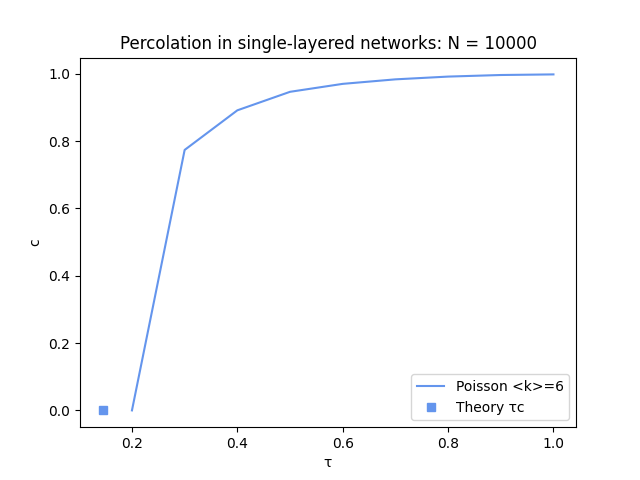
\includegraphics[width=\linewidth]{SIM/Poisson-k6_nodes10000_it10000}\caption{Poisson: $k=6$}
                \label{fig:sim_poisson_k_6}
                \end{figure}
            \end{minipage}
            \hspace{0.05\linewidth}
            \begin{minipage}{0.45\linewidth}
                \begin{figure}[H]
                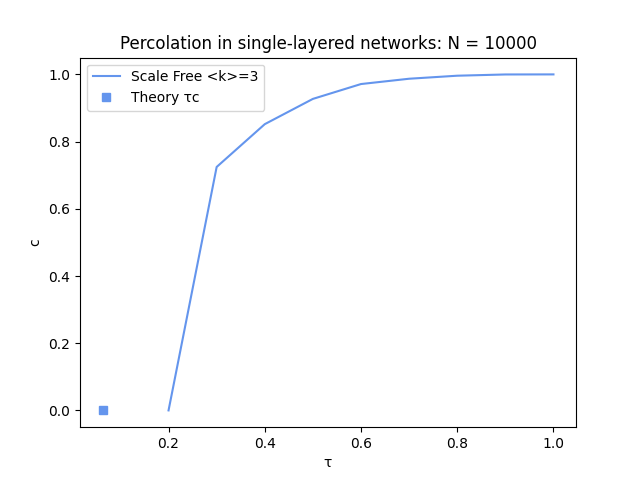
\includegraphics[width=\linewidth]{SIM/ScaleFree-k3_nodes10000_it10000}\caption{Scale-Free: $k=3$}
                \label{fig:sim_scale_free_k_3}
                \end{figure}
            \end{minipage}
            \caption{Valutazione della probabilità di percolazione al variare della tipologia di grafo e del numero di nodi,
            con $n=10000$ e 10000 iterazioni}
        \end{minipage}
    \end{figure}

    \begin{figure}[H]
        \begin{minipage}{\linewidth}
            \centering
            \begin{minipage}{0.45\linewidth}
                \begin{figure}[H]
                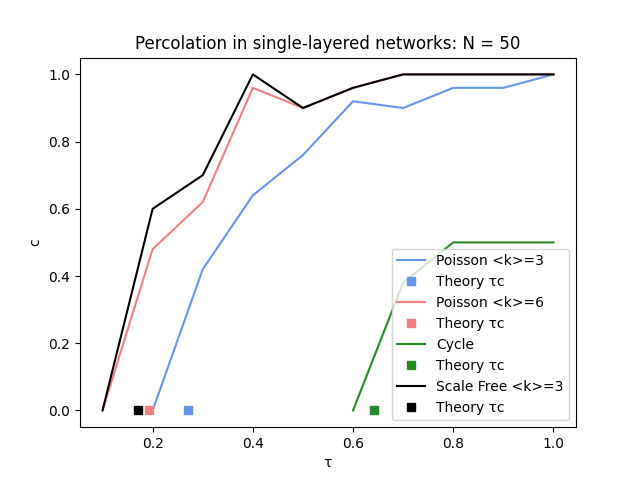
\includegraphics[width=\linewidth]{SIM/tcs-nodes50_it10000}\caption{Valutazione della probabilità di percolazione al variare della tipologia di grafo e del numero di nodi}
                \label{fig:sim_tcs_nodes_50}
                \end{figure}
            \end{minipage}
            \hspace{0.05\linewidth}
            \begin{minipage}{0.45\linewidth}
                \begin{figure}[H]
                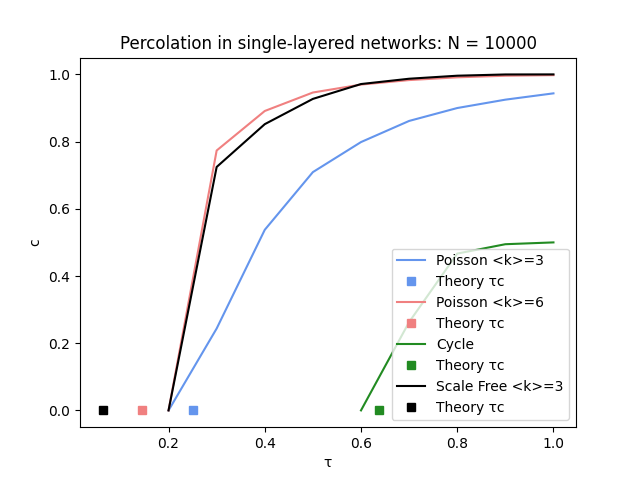
\includegraphics[width=\linewidth]{SIM/tcs-nodes10000_it10000}\caption{Valutazione della probabilità di percolazione al variare della tipologia di grafo e del numero di nodi}
                \label{fig:sim_tcs_nodes_10000}
                \end{figure}
            \end{minipage}
            \caption{Valutazione della probabilità di percolazione al variare della tipologia di grafo e del numero di nodi}
        \end{minipage}
    \end{figure}

\subsection{Infezione percezione del rischio}\label{subsec:app-infezione-con-la-percezione-del-rischio}
    \begin{figure}[H]
        \begin{minipage}{\linewidth}
            \centering
            \begin{minipage}{0.45\linewidth}
                \begin{figure}
                    \includegraphics[width=\linewidth]{PERC/Cycle-nodes50_it10000}\caption{Self percolation Cycle with $k=2$}
                    \label{fig:perc_cycle_nodes_50}
                \end{figure}
            \end{minipage}
            \hspace{0.05\linewidth}
            \begin{minipage}{0.45\linewidth}
                \begin{figure}
                    \includegraphics[width=\linewidth]{PERC/Poisson-k3_nodes50_it10000}\caption{Self percolation Poisson with $k=3$}
                    \label{fig:perc_poisson_k_3_nodes_50}
                \end{figure}
            \end{minipage}
            \begin{minipage}{0.45\linewidth}
                \begin{figure}
                    \includegraphics[width=\linewidth]{PERC/ScaleFree-k3_nodes50_it10000}\caption{Self percolation Scale-Free with $k=3$}
                    \label{fig:perc_scale_free_k_3_nodes_50}
                \end{figure}
            \end{minipage}
            \caption{Confronto self percolation and simulation con $n=50$ e 10000 iterazioni}
        \end{minipage}
    \end{figure}

    \begin{figure}[H]
        \begin{minipage}{\linewidth}
            \centering
            \begin{minipage}{0.45\linewidth}
                \begin{figure}
                    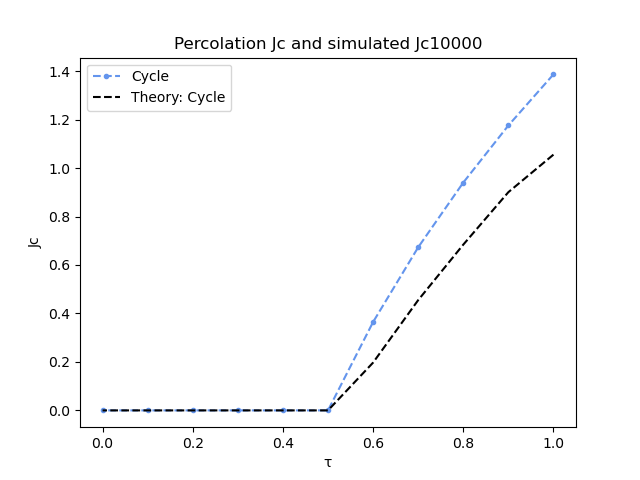
\includegraphics[width=\linewidth]{PERC/Cycle-nodes10000_it100}\caption{Cycle: $k=2$}
                    \label{fig:perc_cycle}
                \end{figure}
            \end{minipage}
            \hspace{0.05\linewidth}
            \begin{minipage}{0.45\linewidth}
                \begin{figure}
                    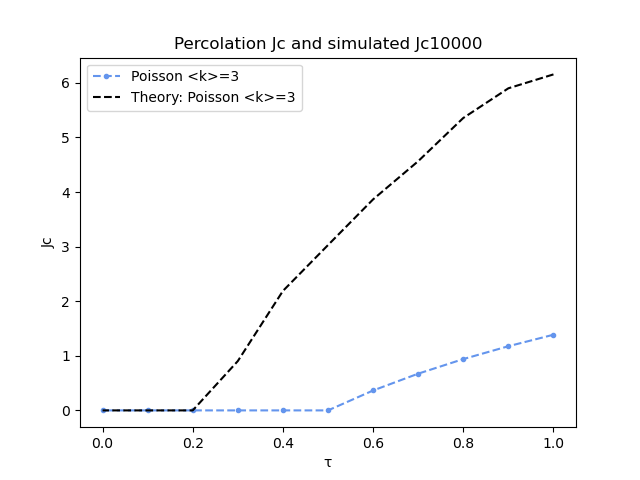
\includegraphics[width=\linewidth]{PERC/Poisson-k3_nodes10000_it100}\caption{Poisson: $k=3$}
                    \label{fig:perc_poisson_k_3}
                \end{figure}
            \end{minipage}
            \begin{minipage}{0.45\linewidth}
                \begin{figure}
                    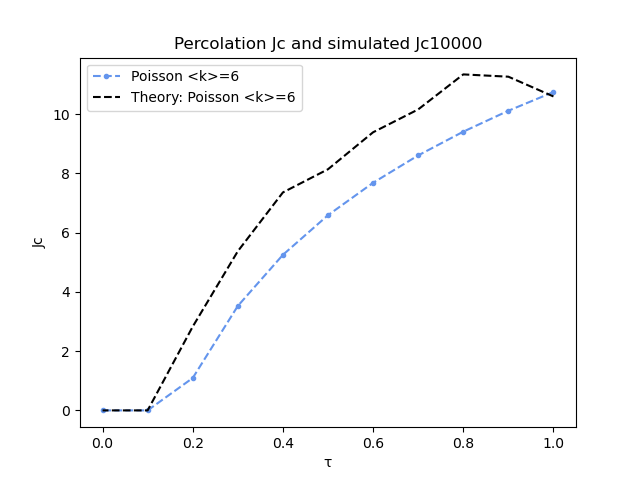
\includegraphics[width=\linewidth]{PERC/Poisson-k6_nodes10000_it100}\caption{Poisson: $k=6$}
                    \label{fig:perc_poisson_k_6}
                \end{figure}
            \end{minipage}
            \hspace{0.05\linewidth}
            \begin{minipage}{0.45\linewidth}
                \begin{figure}
                    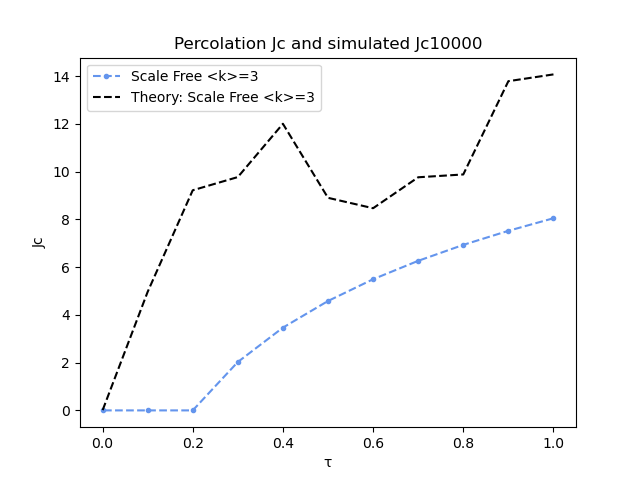
\includegraphics[width=\linewidth]{PERC/ScaleFree-k3_nodes10000_it100}\caption{Scale-Free: $k=3$}
                    \label{fig:perc_scale_free_k_3}
                \end{figure}
            \end{minipage}
            \caption{Confronto self percolation and simulation con $n=10000$ e 100 iterazioni}
        \end{minipage}
    \end{figure}

    \begin{figure}[H]
        \begin{minipage}{\linewidth}
            \centering
            \begin{minipage}{0.45\linewidth}
                \begin{figure}
                    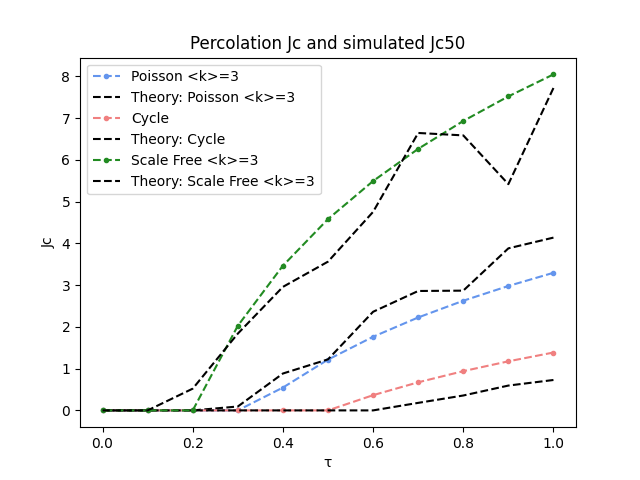
\includegraphics[width=\linewidth]{PERC/percjcs-k3_nodes50_it10000}\caption{Confronto self percolation and simulation con $n=50$ e 10000 iterazioni}
                    \label{fig:perc_jcs_k_3_nodes_50}
                \end{figure}
            \end{minipage}
            \hspace{0.05\linewidth}
            \begin{minipage}{0.45\linewidth}
                \begin{figure}
                    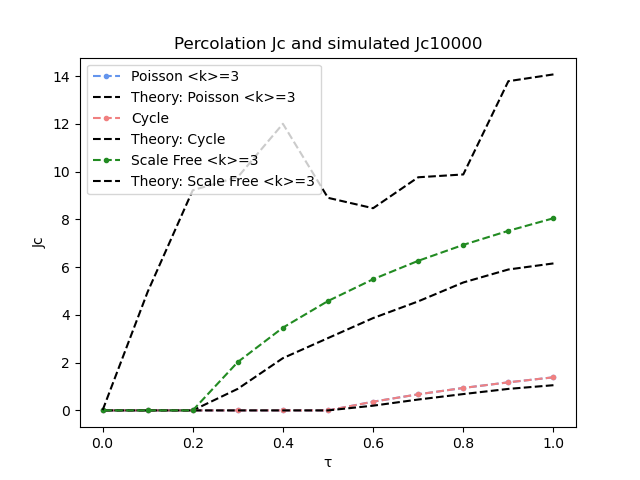
\includegraphics[width=\linewidth]{PERC/percjcs-k3_nodes10000_it100}\caption{Confronto self percolation and simulation con $n=10000$ e 100 iterazioni}
                    \label{fig:perc_jcs_k_3_nodes_10000}
                \end{figure}
            \end{minipage}
            \begin{minipage}{0.45\linewidth}
                \begin{figure}
                    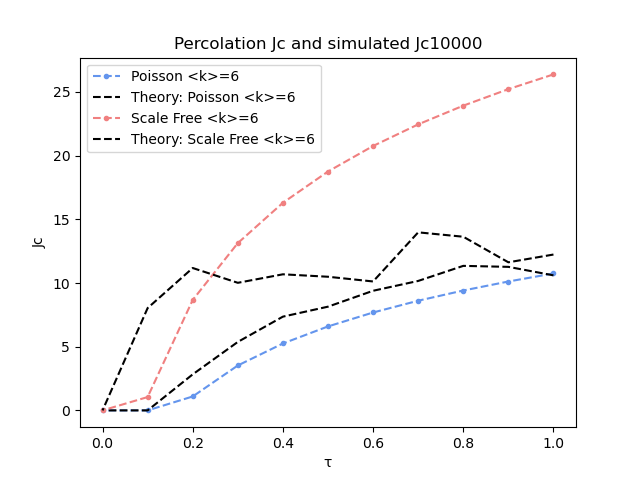
\includegraphics[width=\linewidth]{PERC/percjcs-k6_nodes10000_it100}\caption{Confronto self percolation and simulation con $n=10000$ e 100 iterazioni}
                    \label{fig:perc_jcs_k_6_nodes_10000}
                \end{figure}
            \end{minipage}
            \caption{Confronto self percolation and simulation con $n=10000$ e 100 iterazioni}
        \end{minipage}
    \end{figure}

\subsection{Multiplex networks}\label{subsec:app-multiplex-networks}
    \begin{figure}[H]
        \begin{minipage}{\linewidth}
            \centering
            \begin{minipage}{0.45\linewidth}
                \begin{figure}
                    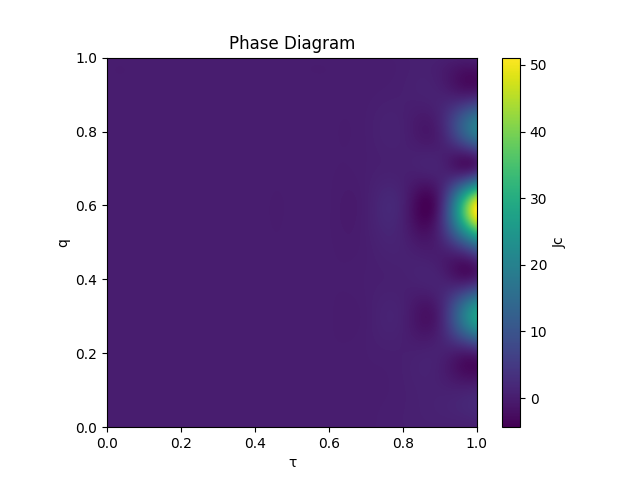
\includegraphics[width=\linewidth]{MUL/Cycle-nodes100_it10000_jminf}\caption{Cycle}
                    \label{fig:mul_cycle}
                \end{figure}
            \end{minipage}
            \hspace{0.05\linewidth}
            \begin{minipage}{0.45\linewidth}
                \begin{figure}
                    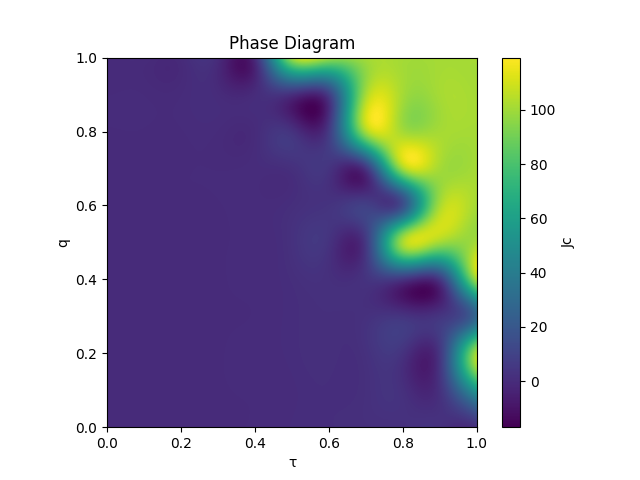
\includegraphics[width=\linewidth]{MUL/Poisson-k3_nodes100_it10000_jminf}\caption{Poisson: $k=3$}
                    \label{fig:mul_poisson_k_3}
                \end{figure}
            \end{minipage}
            \begin{minipage}{0.45\linewidth}
                \begin{figure}
                    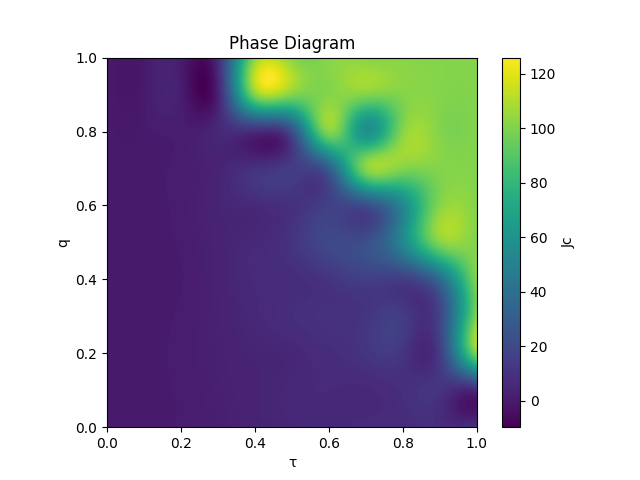
\includegraphics[width=\linewidth]{MUL/ScaleFree-k3_nodes100_it10000_jminf}\caption{Scale-Free: $k=3$}
                    \label{fig:mul_scale_free_k_3}
                \end{figure}
            \end{minipage}
            \caption{Diagramma di fase al variare di $q$ e $\tau$ con $n=100$ e 10000 iterazioni. $J_{\max}=\inf$}
        \end{minipage}
    \end{figure}

    \begin{figure}[H]
        \begin{minipage}{\linewidth}
            \centering
            \begin{minipage}{0.45\linewidth}
                \begin{figure}
                    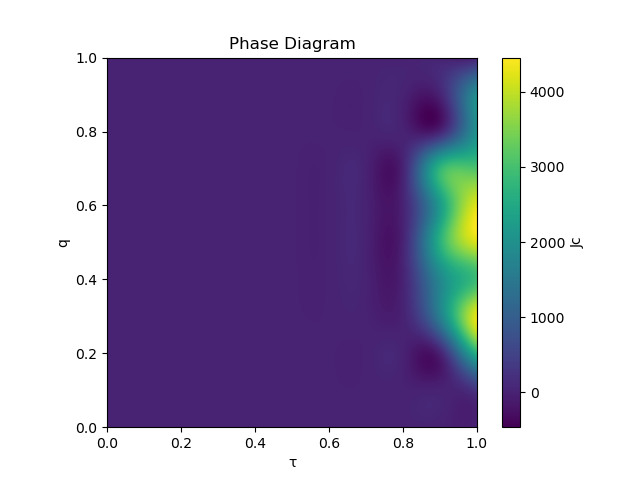
\includegraphics[width=\linewidth]{MUL/Cycle-nodes10000_it100_jminf}\caption{Cycle}
                    \label{fig:mul_cycle_nodes_10000}
                \end{figure}
            \end{minipage}
            \hspace{0.05\linewidth}
            \begin{minipage}{0.45\linewidth}
                \begin{figure}
                    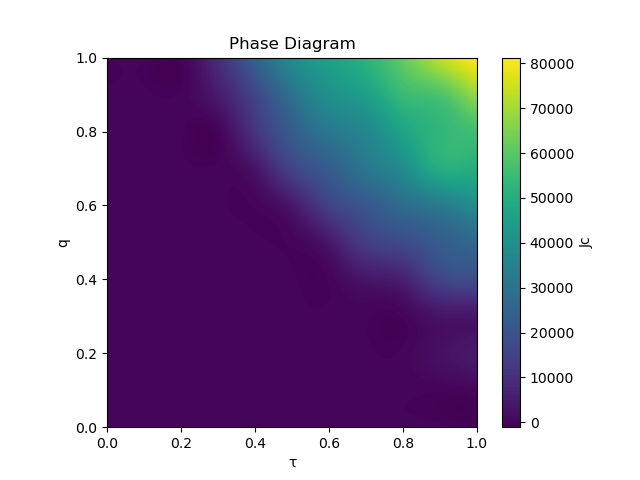
\includegraphics[width=\linewidth]{MUL/Poisson-k3_nodes10000_it100_jminf}\caption{Poisson: $k=3$}
                    \label{fig:mul_poisson_k_3_nodes_10000}
                \end{figure}
            \end{minipage}
            \begin{minipage}{0.45\linewidth}
                \begin{figure}
                    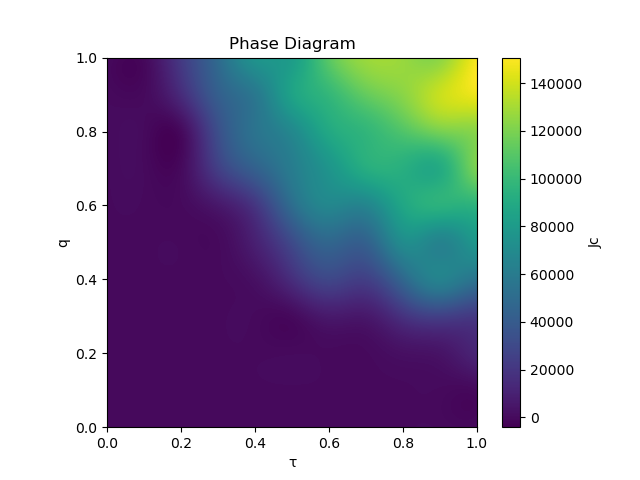
\includegraphics[width=\linewidth]{MUL/Poisson-k6_nodes10000_it100_jminf}\caption{Poisson: $k=6$}
                    \label{fig:mul_poisson_k_6_nodes_10000}
                \end{figure}
            \end{minipage}
            \hspace{0.05\linewidth}
            \begin{minipage}{0.45\linewidth}
                \begin{figure}
                    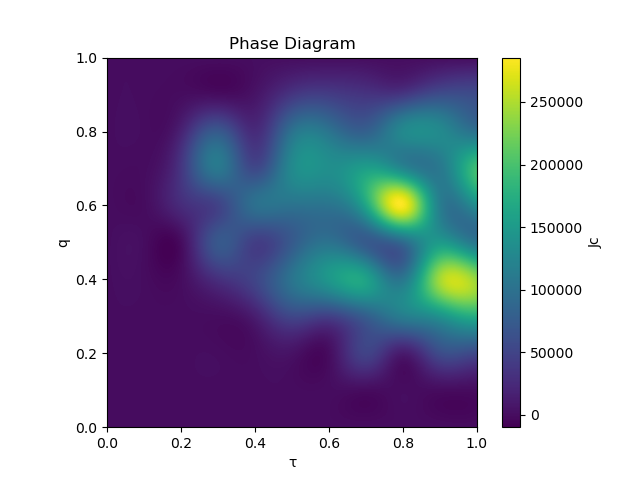
\includegraphics[width=\linewidth]{MUL/ScaleFree-k3_nodes10000_it100_jminf}\caption{Scale-Free: $k=3$}
                    \label{fig:mul_scale_free_k_3_nodes_10000}
                \end{figure}
            \end{minipage}
            \begin{minipage}{0.45\linewidth}
                \begin{figure}
                    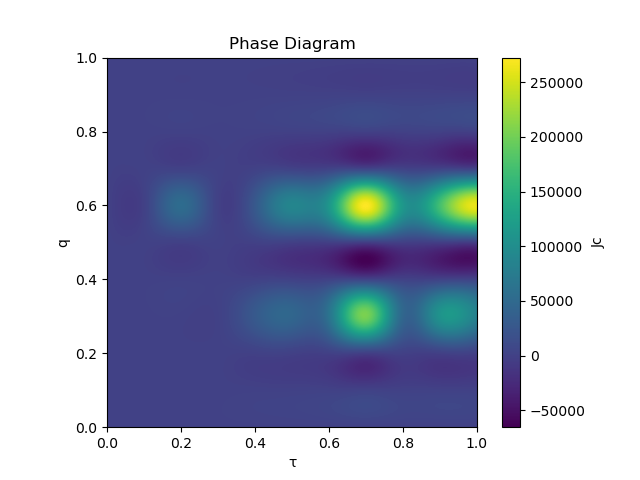
\includegraphics[width=\linewidth]{MUL/ScaleFree-k6_nodes10000_it100_jminf}\caption{Scale-Free: $k=6$}
                    \label{fig:mul_scale_free_k_6_nodes_10000}
                \end{figure}
            \end{minipage}
            \hspace{0.05\linewidth}
            \begin{minipage}{0.45\linewidth}
                \begin{figure}
                    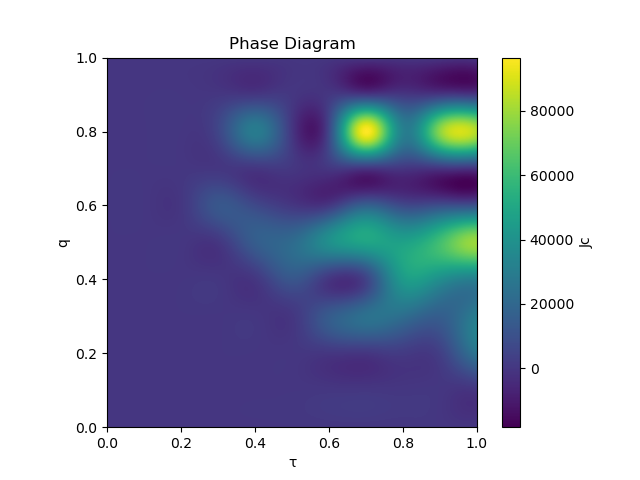
\includegraphics[width=\linewidth]{MUL/Poisson-k6+ScaleFree-k6_nodes10000_it100_jminf}\caption{PG:Poisson: $k=6$ + VG:Scale-Free: $k=6$}
                    \label{fig:mul_poisson_k_6_scale_free_k_6_nodes_10000}
                \end{figure}
            \end{minipage}
            \caption{Diagramma di fase al variare di $q$ e $\tau$ con $n=10000$ e 100 iterazioni. $J_{\max}=\inf$}
        \end{minipage}
    \end{figure}

    \begin{figure}[H]
        \begin{minipage}{\linewidth}
            \centering
            \begin{minipage}{0.45\linewidth}
                \begin{figure}
                    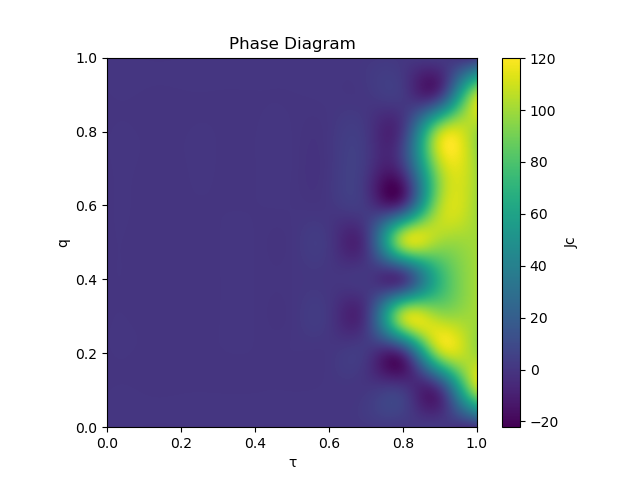
\includegraphics[width=\linewidth]{MUL/Cycle-nodes10000_it100_jm100}\caption{Cycle}
                    \label{fig:mul_cycle_nodes_10000_jm_100}
                \end{figure}
            \end{minipage}
            \hspace{0.05\linewidth}
            \begin{minipage}{0.45\linewidth}
                \begin{figure}
                    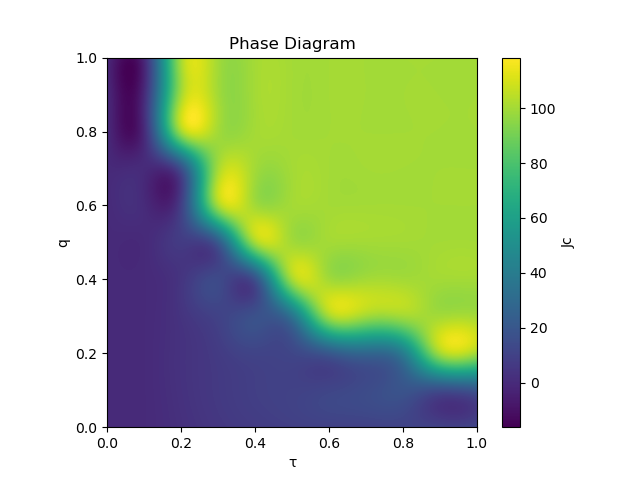
\includegraphics[width=\linewidth]{MUL/Poisson-k6_nodes10000_it100_jm100}\caption{Poisson: $k=3$}
                    \label{fig:mul_poisson_k_3_nodes_10000_jm_100}
                \end{figure}
            \end{minipage}
            \hspace{0.05\linewidth}
            \begin{minipage}{0.45\linewidth}
                \begin{figure}
                    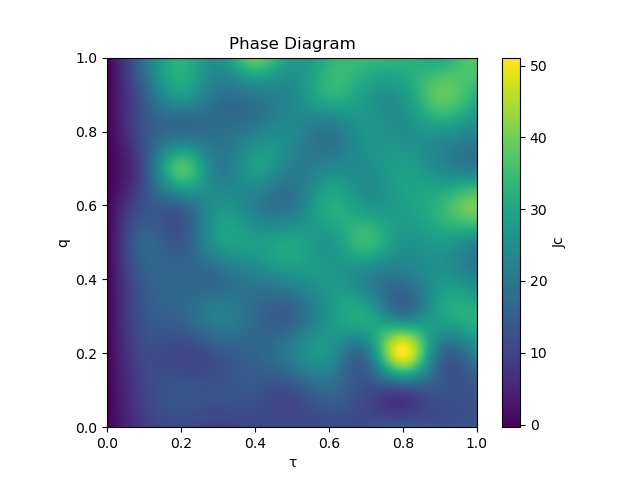
\includegraphics[width=\linewidth]{MUL/ScaleFree-k6_nodes10000_it100_jm100}\caption{Scale-Free: $k=6$}
                    \label{fig:mul_scale_free_k_6_nodes_10000_jm_100}
                \end{figure}
            \end{minipage}
            \begin{minipage}{0.45\linewidth}
                \begin{figure}
                    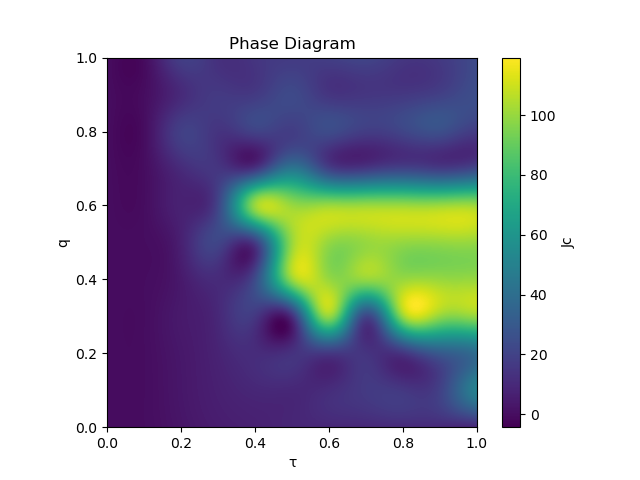
\includegraphics[width=\linewidth]{MUL/Poisson-k6+ScaleFree-k6_nodes_10000_it100_jm100}\caption{PG:Poisson: $k=6$ + VG:Scale-Free: $k=6$}
                    \label{fig:mul_poisson_k_6_scale_free_k_6_nodes_10000_jm_100}
                \end{figure}
            \end{minipage}
            \caption{Diagramma di fase al variare di $q$ e $\tau$ con $n=10000$ e 100 iterazioni. $J_{\max}=100$}
        \end{minipage}
    \end{figure}
